\section{Expedition Proceedings}


    \begin{marginfigure}
\checkoddpage \ifoddpage \forcerectofloat \else \forceversofloat \fi
\centering
 \frame{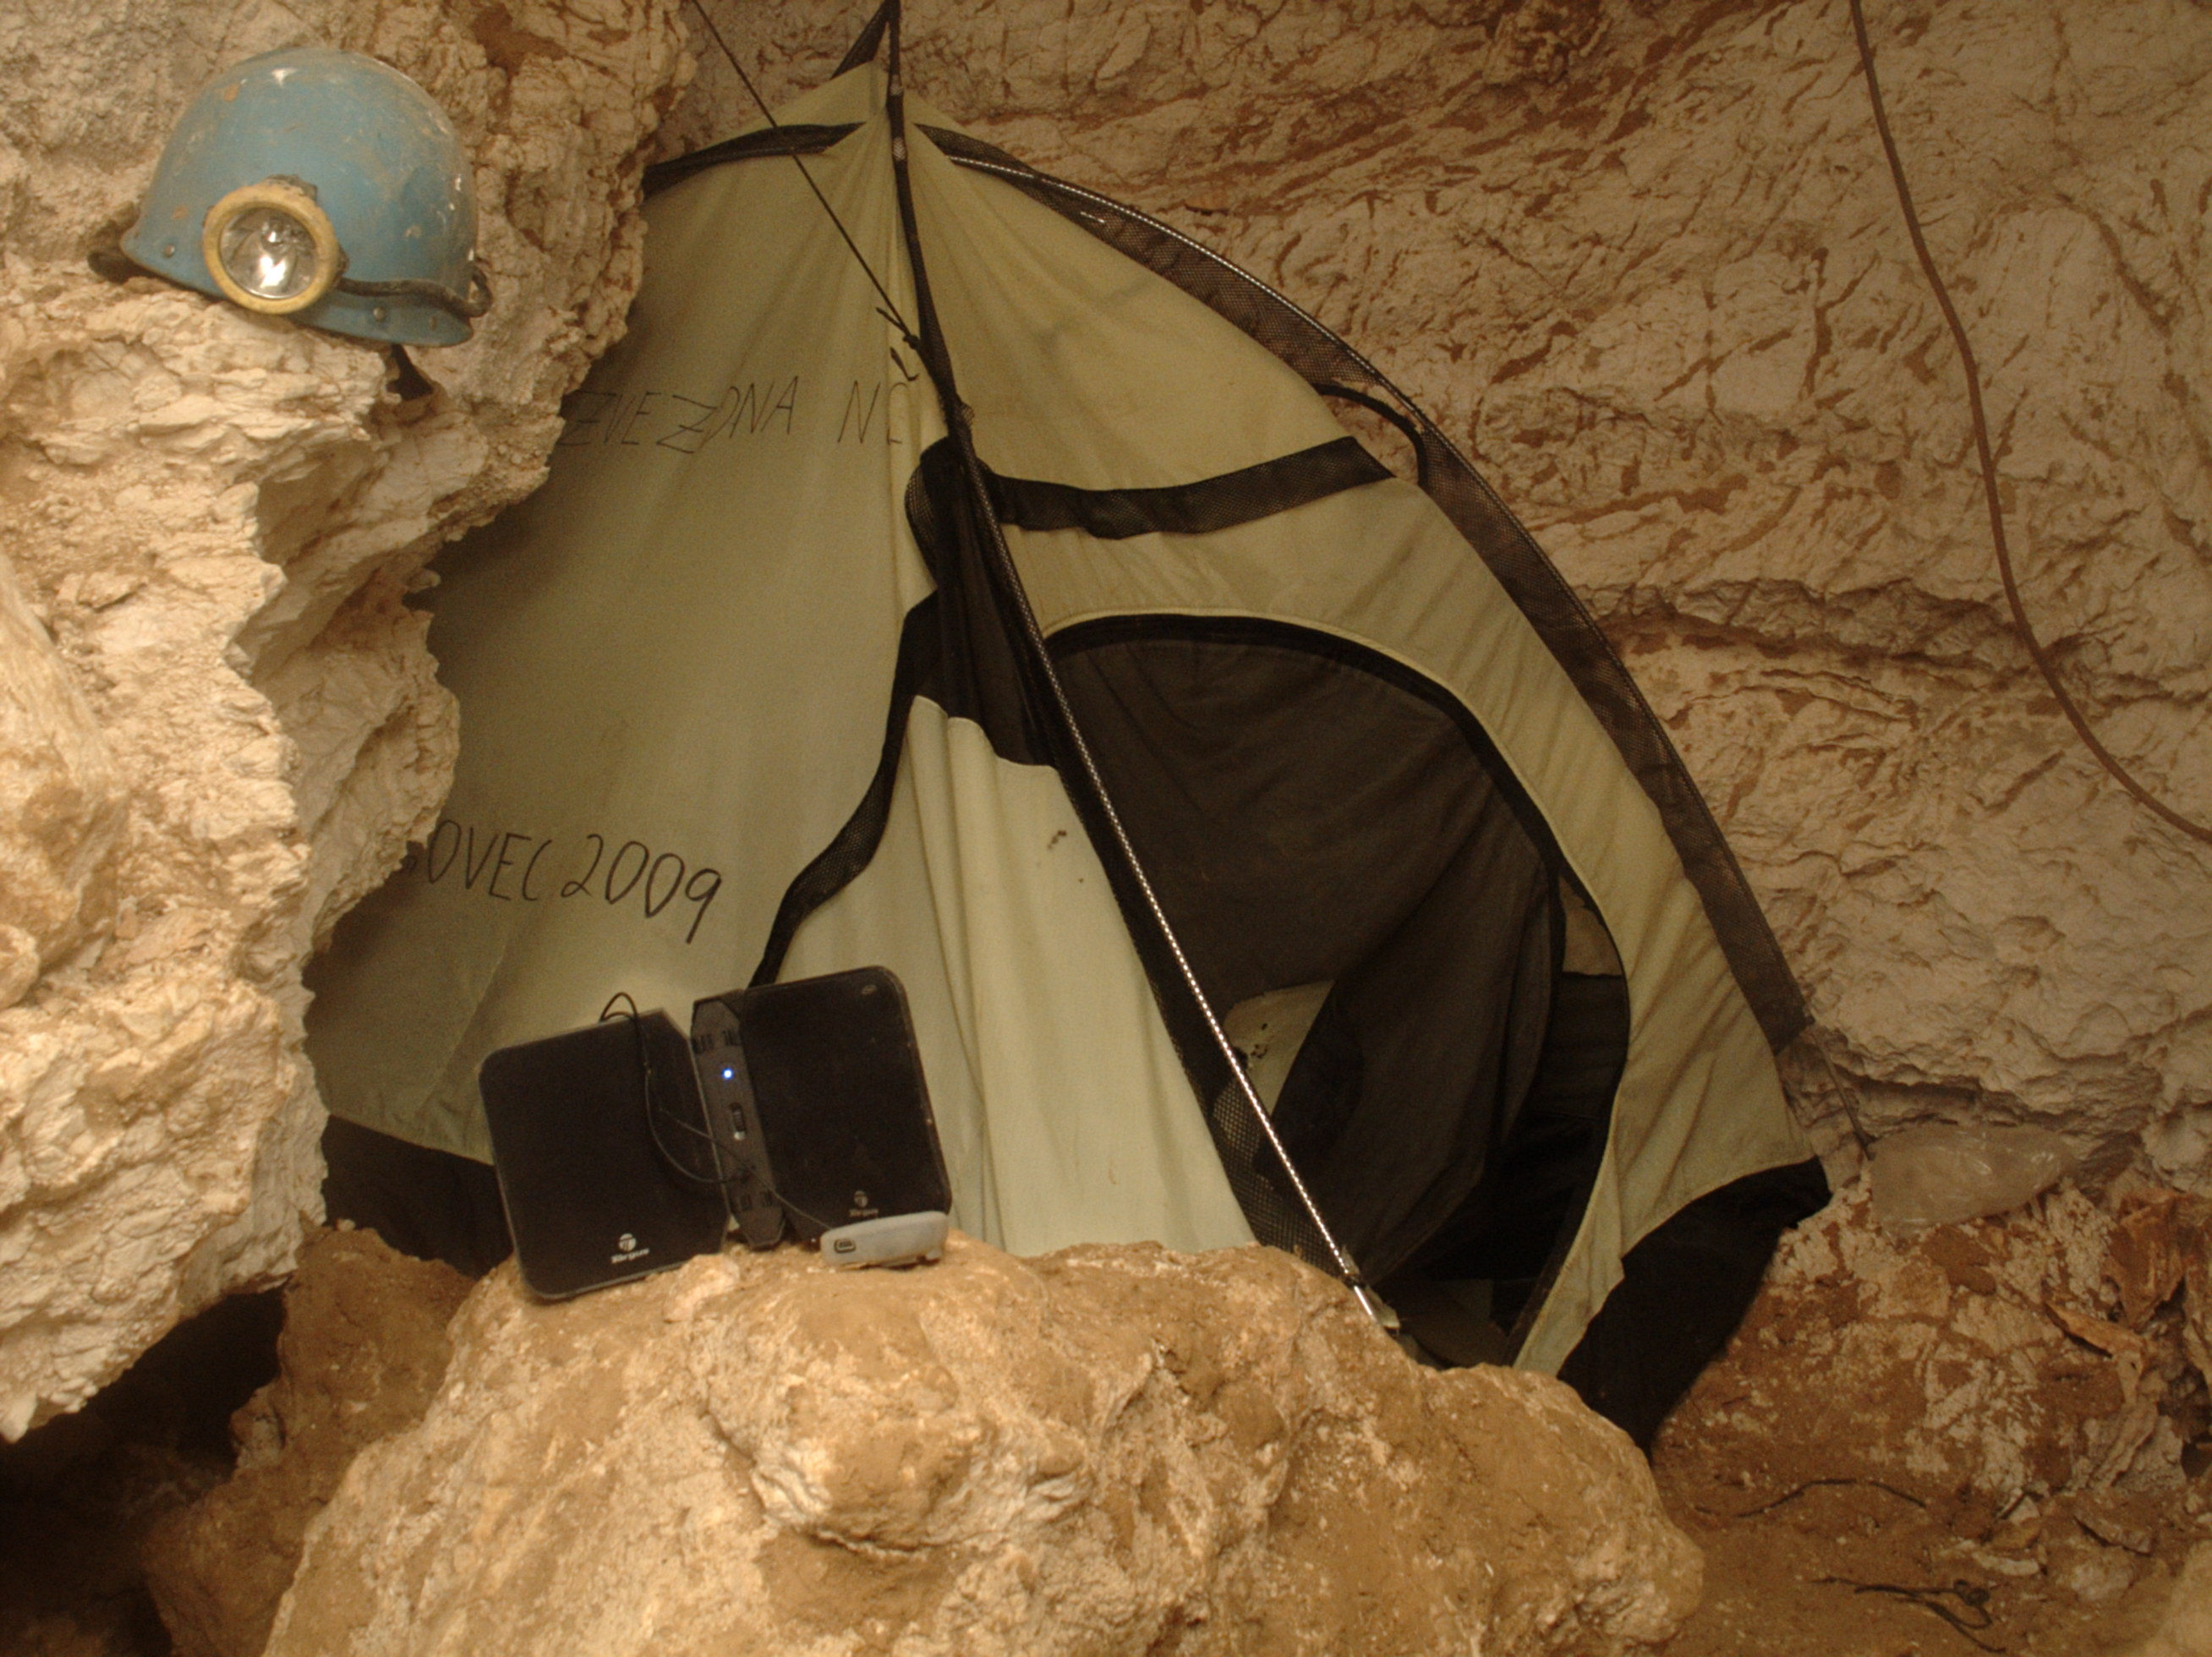
\includegraphics[width=\linewidth]{2009/proceedings/2009-08-05-20.29.00 - Jarvist Frost - Canon Powershot G5 - tent in metal camp--orig.jpg}} 
 \caption{The tent and sound system in place at \protect\passage{Metal Camp}. \pic{Jarvist Frost}}
 \label{metal camp tent}
\end{marginfigure}

\tweet{2:19 PM Jul 30, 2009}{Silos windows pushed to base of ~30m pitch JH/MF. 5 bags UG camp stuff to traverse chamb and CK rig JKP/TS. S1 opened for business.}

We installed \passage{Metal Camp} at -254 m in an until-now torturous parallel shaft
series, \passage{Captain Kangaroo}. Thirty-two people-nights were spent at the two man underground camp,
with two twelve hour shifts of hot-bedding. Exploration in this section
of \passage{Vrtnarija} was split between looking at
climbing leads in the hope of connecting to \passage{M2}, and pushing the
\passage{Dark Tranquillity} series downwards. The majority of the climbing
was done via bounce trips from the surface, and also as `light days' for
people on their way out from camp. All the deep pushing was done from
the camp downwards. Total amount of caving was 98 people trips,
including camping trips.

In 2008 we had left the developing pitch series at the bottom of
\passage{Dark Tranquillity}, as this level in \passage{Vrtnarija} had now
dropped below the known extent of \passage{M2}; the main expedition aim in
2009 was to try and connect \passage{Vrtnarija} to \passage{Sistem Migovec}. Cave
exploration progressed quickly and easily, with depth building at the
rate at which pitches could be safely rigged, gardened and surveyed.

Within two weeks of the caving commencing we had bottomed \passage{Happy
Monday} (P81 m), with the resulting survey data indicating an almost
inevitable intersection with the horizontal development at -550 m in
\passage{Vrtnarija} (\passage{Friendship Gallery}). The next team down pushed
through the terrifying boulder choke at the floor of the chamber
(\passage{Hanging Garden}), gained a well developed rift with phreatic
crawlspace at the top, and \bignote{pushed downwards until they found an old bolt}
just beyond a small confluence.

Plotting the data back on the mountain top it was clear that they had
intersected \passage{Falls Road}, a set of tight active rifts accessed
just below \passage{Friendship Gallery}. The next trip into the cave went
via the main pitch series and dropped a rope down from this \passage{Prima
Junction}, intersecting the rigging left by the previous push. Strangely
the 2001/2003 explorers had missed the lead towards `\passage{Happy
Monday}', even though the end of the large rift forms one of the
original rebelay bolts for the confluence pitch.

    \begin{marginfigure}
\checkoddpage \ifoddpage \forcerectofloat \else \forceversofloat \fi
\centering
 \frame{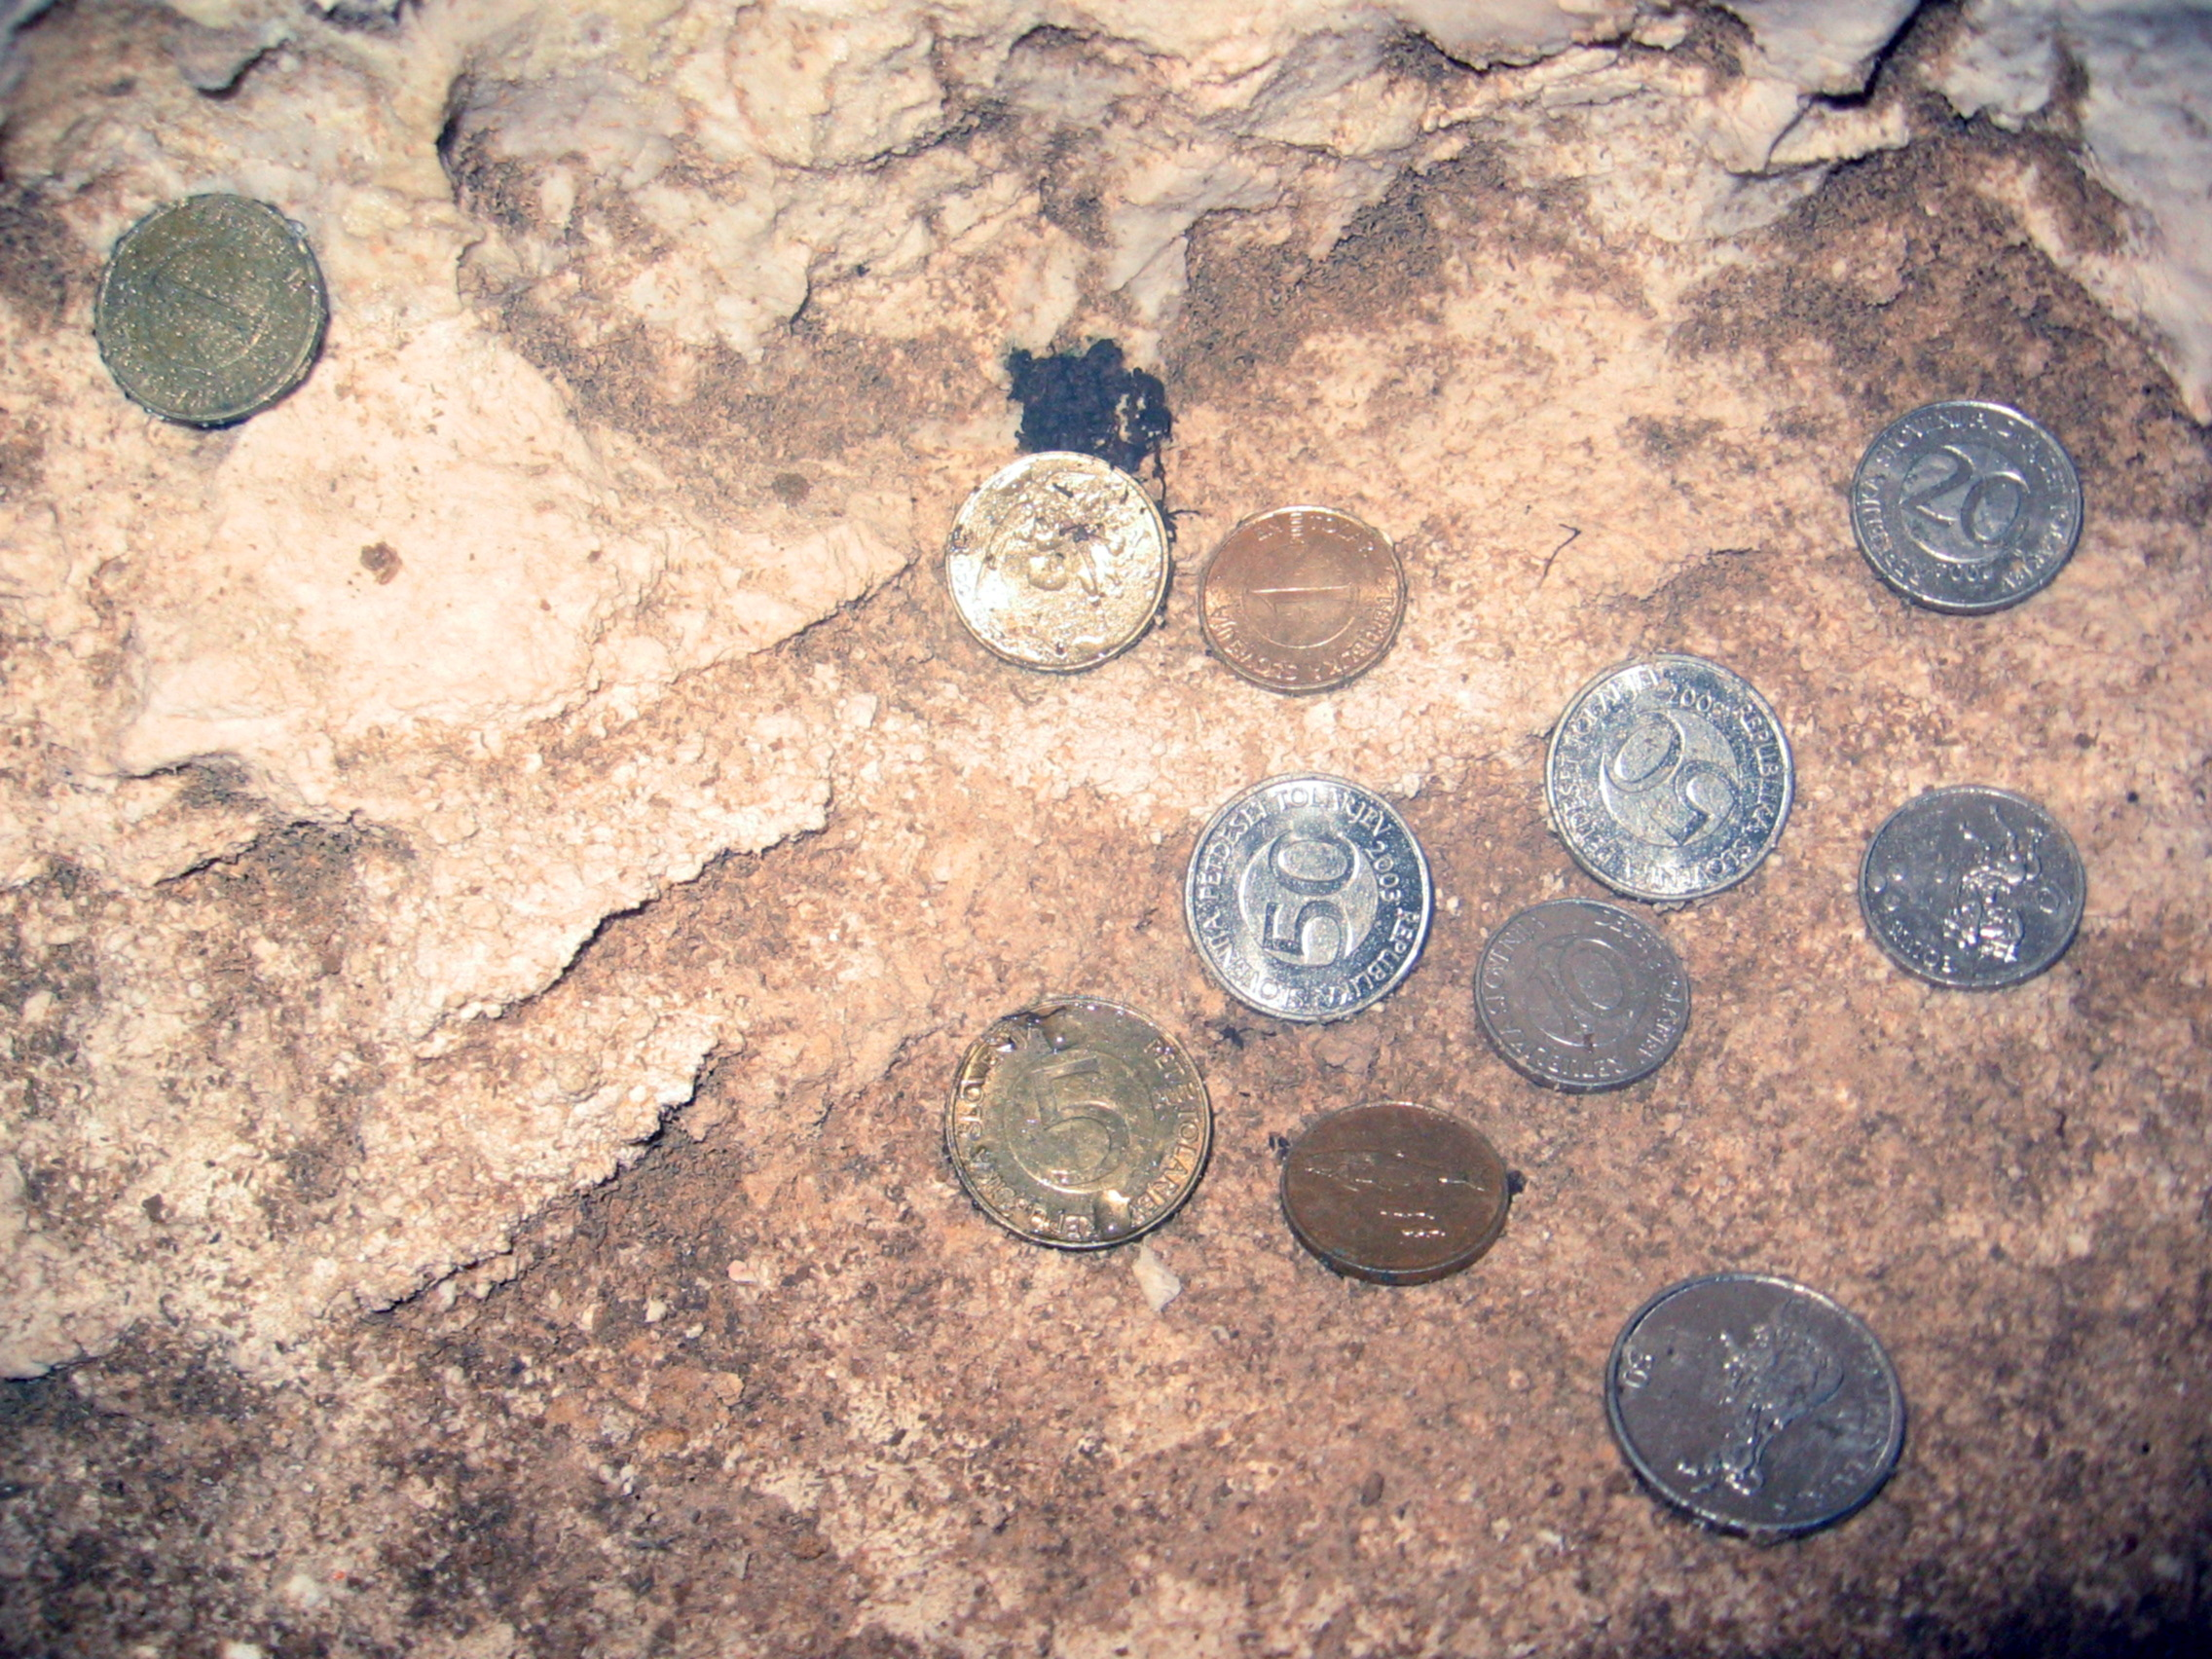
\includegraphics[width=\linewidth]{2009/proceedings/2009-08-15-23.53.37 - Jana Carga - Canon Powershot A520 - Fistful of Tolars - badly fogged lens2--orig.jpg}} 
 \caption{After connecting the \passage{Captain Kangaroo} branch and \passage{Falls Road}, the expedition descended the main \passage{Vrtnarija} pitch series to reach the connection point from \passage{Friendship Gallery}, which includes the pitch \passage{Fistful of Tolars} featuring physical cash at the pitch-head. \pic{Jana Čarga}}
 \label{fistful of tolars}
\end{marginfigure}

The last camping trip saw an epic list of `must do this year' tasks,
dropping into the newly discovered \passage{Tolminska Korita} via the
easily passed main pitch series, taking pictures of new discoveries and
undocumented pitches along the way, recording the new discoveries from
\passage{Falls road} back to \passage{Walk the Line}, resting overnight at
camp, then descending to the connection point once more to finish off
the survey, investigate the `\passage{Muddy Window}' phreatic passage 10 m
above the floor of \passage{Happy Monday}, and derig back to camp before
resting again and then striking camp in the morning.

\subsection{Climbs near Camp}

`\passage{Metal Aven}' (C+30 m) still has places left to scale, but appears
from the survey to reconnect to an earlier part in the fault (we
believe) controlled cave development in this region.

`\passage{KETI}' (C+23 m) consisted of an extremely exposed climb (across a
65 m pitch) to gain a rift jammed with unstable boulders which were
traversed to eventually realise a non-human sized connection to a low
part of \passage{Metal Aven}. We had hoped that this rift would trend
South, towards \passage{M2}, but instead it almost immediately doubled-back on
itself in a North-East direction.


    \begin{marginfigure}
\checkoddpage \ifoddpage \forcerectofloat \else \forceversofloat \fi
\centering
 \frame{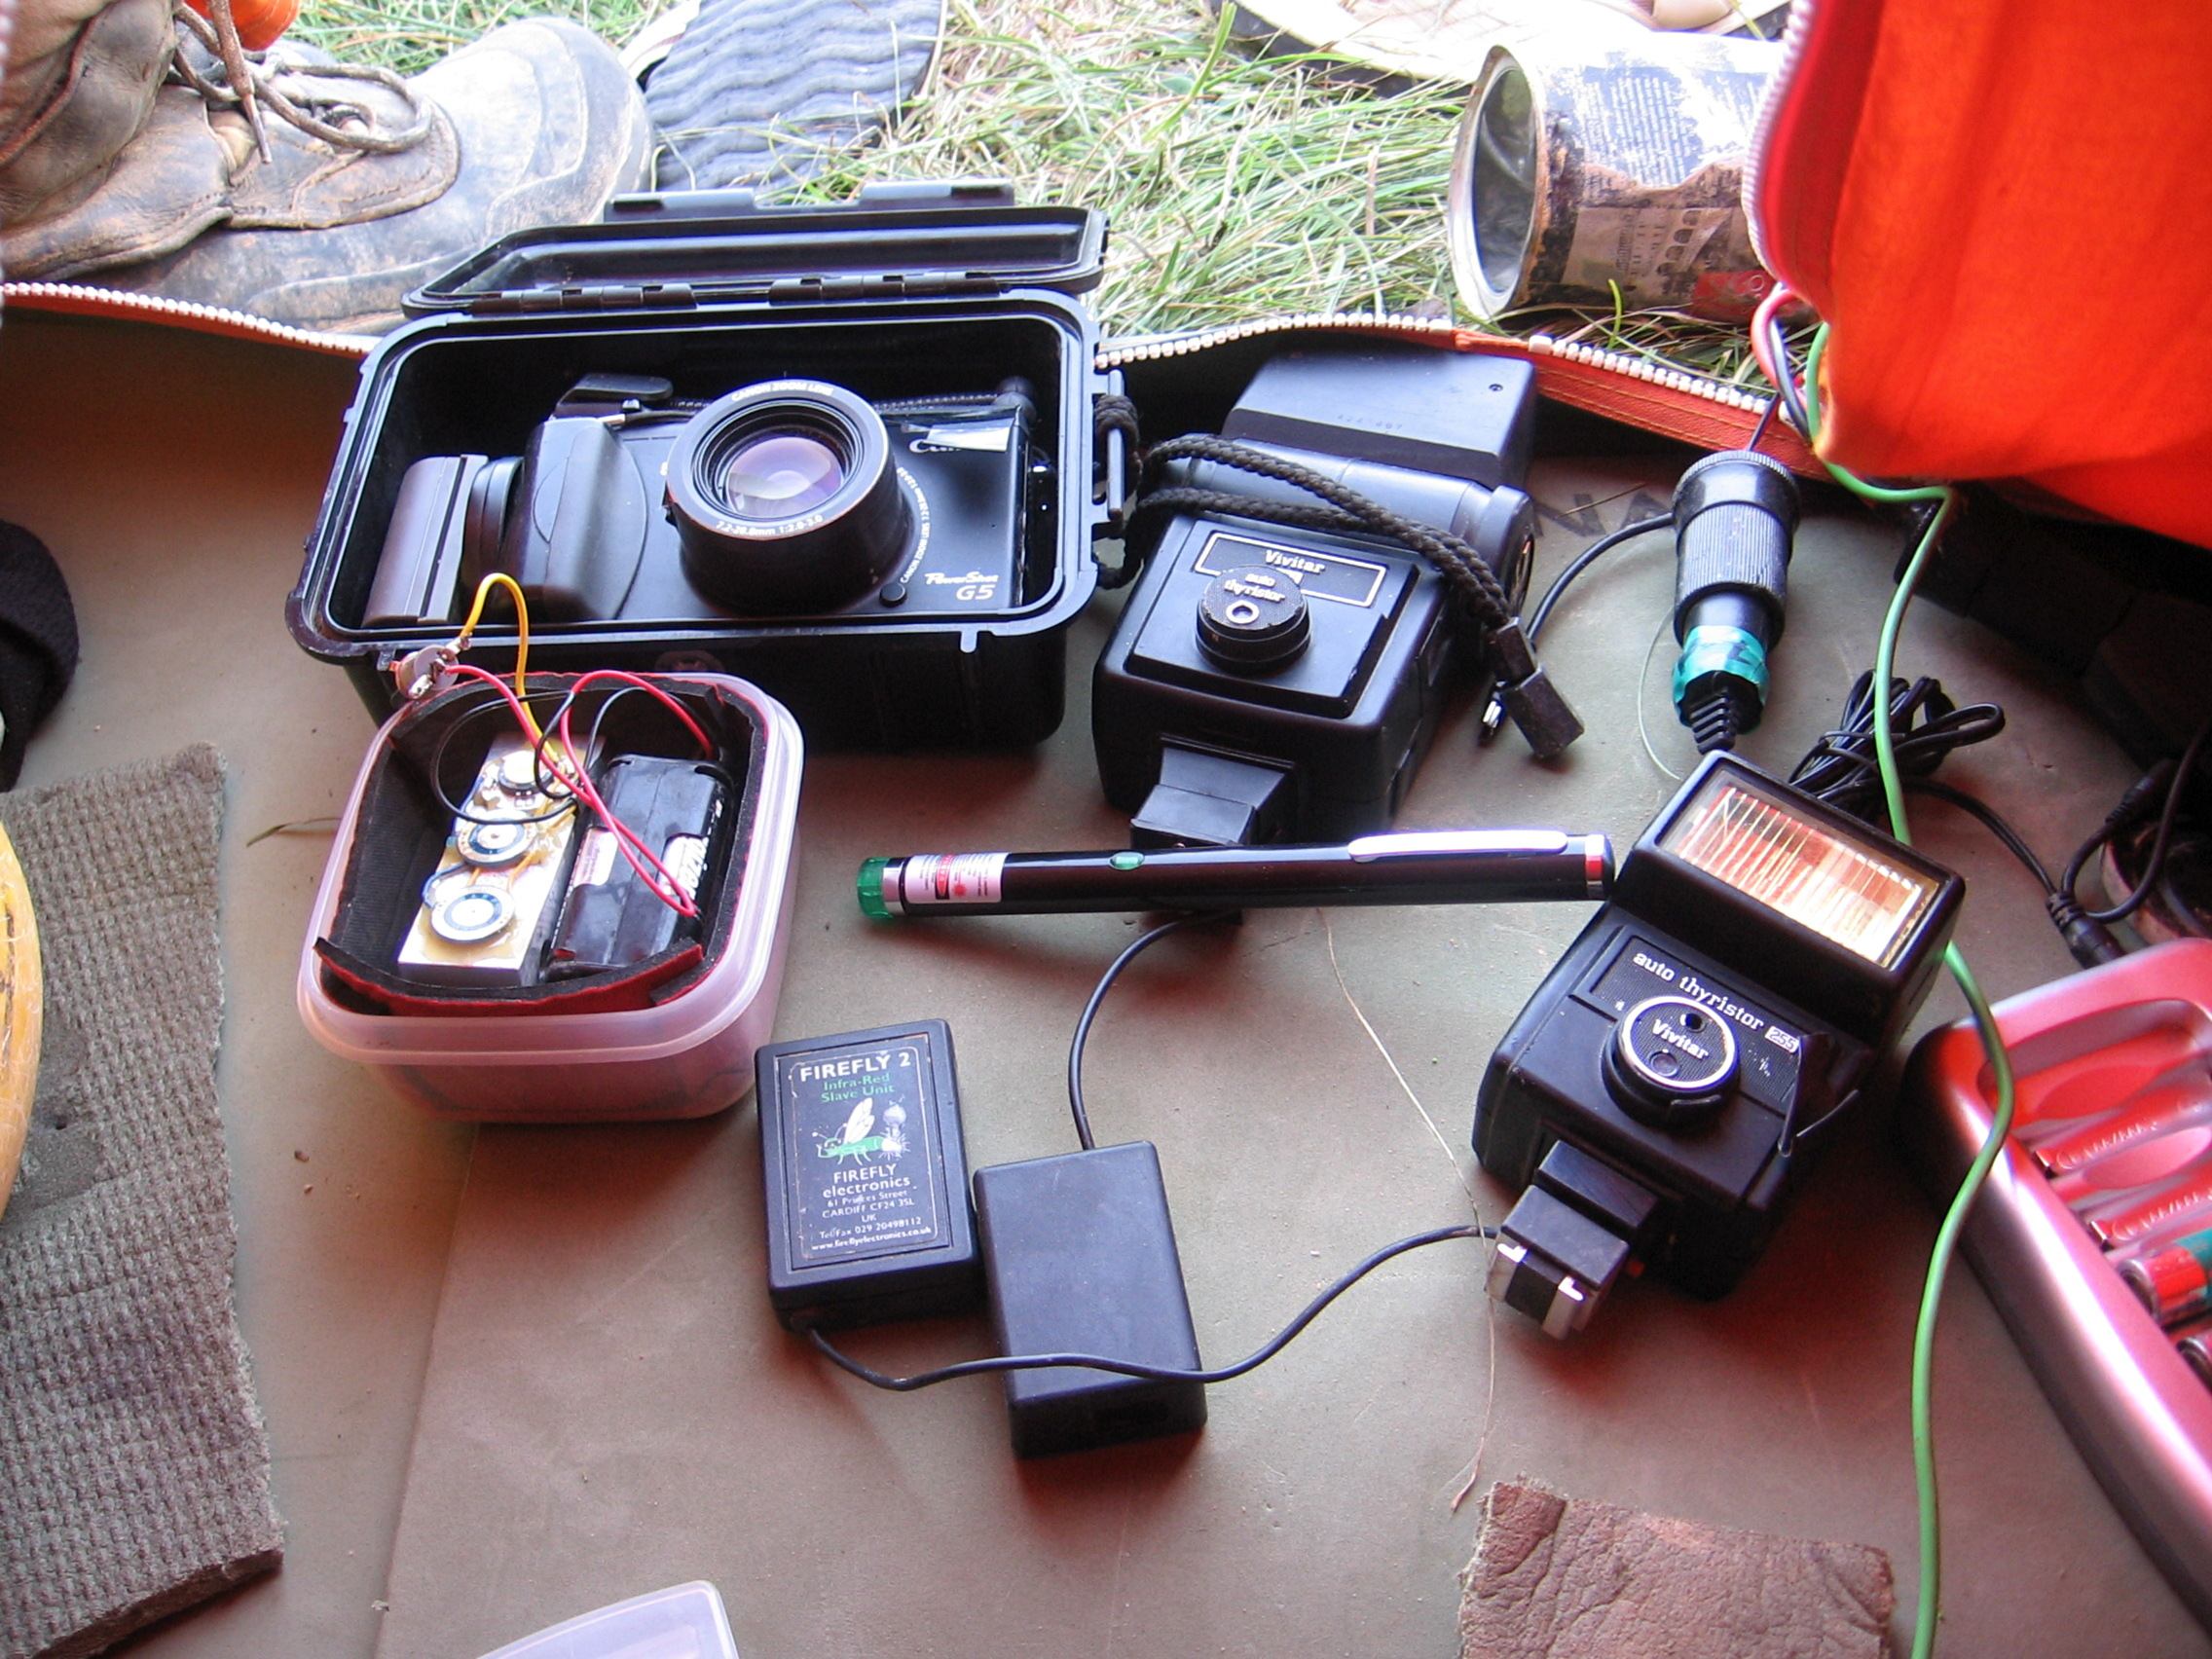
\includegraphics[width=\linewidth]{2009/proceedings/2009-08-12-18.11.15 - Jarvist Frost - Canon Powershot A520 - Preparing photo gear for last camping trip--orig.jpg}} 
 \caption{Photography gear is vital to bringing cave exploration documentation to life. Without the efforts of underground photographers, this would be a much less interesting publication. \pic{Jarvist Frost}}
 \label{photo kit 2009}
\end{marginfigure}



`\passage{Ride the Lightning}' (C+16 m), a climb of the twin shaft to
\passage{Kill'em All} pitch, gained a small section of passage which ended
at a pitch, estimated as being 30 m deep. Lack of gear and time
prevented its exploration, though the survey indicates it may be in the
vicinity of the bottom of \passage{Dangermouse} (2009, P52 m), and may yet
hold the key to bypassing the immature and unpassably small rift which
the \passage{Dangermouse} water disappeared down.

\subsection{Deep Push to \passage{Republika}}

A lightweight bounce-push was made to -734 m to look at a major lead
left at the end of the 2004 deep camping expedition. Due to a
miscommunication during 2004, the upstream `tube tunnel' sized passage
was left unexplored until the last camping trip, everyone having assumed
that '\passage{Red Cow}' died with a sump. This was pushed upstream over a few small
cascades to reach a large watershed, \passage{Republica Palma de Coco}\sidenote{'Republika Palma de Coco' is a song by Slovenian artist Iztok Mlakar from the album 'Štorije In Baldorije', released in the early 1990s. Any student who joins ICCC for more than a trip or two will inevitably hear the song, long before they first step foot in Slovenia},
with the water entering from a high aven, literally splitting on a
triangular rock. It is hypothesised that this water could be coming from
\passage{Tolminska Korita}, 130 m away in both vertical and horizontal
directions. From the watershed, the new passage was followed downstream
to a 13 m pitch which was rigged with the tiny amount of gear that the
party had with them. This took them to a large active rift development,
with an unplumbed depth estimated at being in the region of 30 m. With
no more rigging gear, they surveyed out. The plan of this area is
interesting, with the two streams describing a crescent, with the end of
the rift in the new area being just 16 m away from the previous sump,
indicating that this sump is almost certainly perched and may feed onto
the same pitch series.

This was an extremely happy discovery for this cave, as the maximum
depth of -802 m is believed to be some 200 m above the shale-band
controlled water-table, and an active pitch has the potential to punch
through the sandy choked passage that otherwise dominate this area of
horizontal development.

\tweet{11:26PM Aug 22, 2009}{Slideshow went well, lovely food put on by the PDT. Made a thousand goodbyes and fled into the night.}


\subsection{October 2009}

A small JSPDT/ICCC team returned to \passage{M2} on a weekend in October.
Chemical persuasion was used to open the terminal rift in the floor,
leading to another small chamber. The phreatic passage further on from
the 2008 climb was dug out and extended to a point estimated at 30 m
from the base of the pitch which marked the end of exploration in 2008.
The wet pitches were derigged on the way out and the cave was left till
summer 2010.